\documentclass{article}
\usepackage[english]{babel}
\usepackage{amsmath}
\usepackage{graphicx}
\usepackage{listings}
\usepackage [margin=0.5in] {geometry}


\begin{document}
\begin{titlepage}
  \begin{center}
    \vspace*{1cm}
    
    \Huge
    \textbf{Matrix Multiplication}
    
    \vspace{0.5cm}
    \LARGE
    PROJECT 3
    
    \vspace{1.5cm}
    
    \textbf{Feiyang Zheng}
    
    \vfill
    
    \vspace{0.8cm}
    
    \Large
    Department of Mathematics\\
    SUSTech\\
    China\\{April 2024}
    
  \end{center}
\end{titlepage}

\section{Introduction}

Matrix multiplication is a fundamental operation in linear algebra. In this project, we will implement a matrix multiplication algorithm in C, then compare their performances with different matrix sizes and different optimization strategy, including different compilation flags, block matrix multiplication, vectorization, loop unrolling and vanilla parellelization. 
\section{Naive Matrix Multiplication}
\subsection{Algorithm}

The code for naive matrix multiplication is as follows:
\begin{verbatim}
void multiply(float* a, float* b, float* result, int n) {
  for (int i = 0; i < n; i++) {
    for (int j = 0; j < n; j++) {
      for (int k = 0; k < n; k++)
        result[i*n + j] += a[i*n + k] * b[k*n + j];
    }
}
}
\end{verbatim}

Instead of using \texttt{float \* \*} 2D array, 1D array is implemented because Prof. Yu claims on C programming class that this can reduce the number of jumping, althogh this is not the case when \texttt{-O3} is enabled, for the sake of simplicity, 1D array is used in this project.
\subsection{Notation}
Throughout this report, the following notation will be used:
\begin{itemize}
  \item $m$ is the height of the matrices.
  \item $n$ is the width of the matrices.
  \item $(i,j)$ is the element in the $i$-th row and $j$-th column of a matrix.
  \item $A$ is the right matrix.
  \item $B$ is the left matrix.
  \item $C$ is the result matrix, such that $C = BA$
\end{itemize}

\subsection{OPENMP}
To parallelize the code, we can use the \texttt{\#pragma omp parallel for} directive to parallelize the outermost loop. \texttt{omp} is a library that allows us to parallelize the code.

\subsection{SIMD}
SIMD (Single Instruction, Multiple Data) is a technique that allows the processor to perform multiple operations in parallel. To enable SIMD, we can use the \texttt{-mavx} flag when compiling the code. The idea is to use one vector \texttt{\_\_m256} or \texttt{\_\_m512} to store multiple floats, and use the \texttt{\_mm256\_load\_ps} function to load a vector from memory. The \texttt{\_mm256\_fmadd\_ps} function can be used to multiply and add two vectors, by doing so, the program reduce the number of instructions, and improve the performance.

\subsection{Flops}
The number of flops is the number of floating-point operations per second. The number of flops can be calculated by the following formula:
$$ \text{flops} = \frac{2\times N ^ 3}{time} $$

\subsection{matrices}
In this project, the matrices are defined as a \texttt{struct} in C, the code is as follows:
\begin{lstlisting}[language=C,breaklines=true,basicstyle=\small,caption={Matrix Struct},captionpos=b]
#define BLOCK\_SIZE 32
typedef struct {
    size_t m;           // Number of rows
    size_t n;           // Number of columns
    size_t m_pad;       // Number of rows padded to multiple of BLOCK\_SIZE
    size_t n_pad;       // Number of columns padded to multiple of BLOCK\_SIZE
    float* array;    // Pointer to the matrix elements
    // floats are stored in column-major order
} Matrix;

Matrix* createMatrix(size_t m, size_t n) {
    Matrix* matrix = (Matrix*)malloc(sizeof(Matrix));
    matrix->m = m;
    matrix->n = n;
    matrix->m_pad = (m + BLOCK\_SIZE-1) & ~(BLOCK\_SIZE-1);
    matrix->n_pad = (n + BLOCK\_SIZE-1) & ~(BLOCK\_SIZE-1);
    matrix->array = (float*)aligned_alloc(32, matrix->m_pad * matrix->n_pad * sizeof(float));
    return matrix;
}
\end{lstlisting}

Here \texttt{BLOCK\_SIZE} is defined as 32, which is the size of the block used in the blocked matrix multiplication algorithm. The matrices are stored in column-major order, and the number of rows and columns are padded to a multiple of 32, because the loop in block verion move the index by 32 each time, thus the size of the matrix must be a multiple of 32, otherwise the program will crash.

\section{Block Matrix Multiplication}
Since the matrices are stored in column major, the innermost loop of the naive matrix multiplication algorithm is not cache friendly. To improve cache performance, we can exchange the loop $k$ and $j$ in the naive matrix multiplication algorithm, resulting better performance. The code for block matrix multiplication is as follows:
\begin{verbatim}
void multiply(float* a, float* b, float* result, int n) {
for (int i = 0; i < n; i++) {
    for (int j = 0; j < n; j++) {
        for (int k = 0; k < n; k++){
            result[i + j*m] += a[i + k*m] * b[j + k*m];
        }
    }
}
}
\end{verbatim}
However, such algorithm is not ideal for further optimization, we will use a similar algorithm called block matrix multiplication in the following sections.

\section{Vectorization}
Vectorization is a technique that allows the processor to perform multiple operations in parallel. My personal computer has an Intel i9-12900HX processor, which supports AVX-256. To enable vectorization, we can use the \texttt{-mavx} flag when compiling the code. 
\subsection{Step by Step Inprovement}
We start with the naive matrix multiplication algorithm, we can apply \texttt{\#pragma omp parallel for} to parallelize the outermost loop. The code is as follows:
\begin{lstlisting}[language=C,breaklines=true,basicstyle=\small,caption={Step by Step Improvement},captionpos=b]
  //step by step
int multiply0(Matrix* A, Matrix* B, Matrix* C) {
    if (A->m != B->n) {
        printf("Error: Matrix dimensions do not match\n");
        return 1;
    }
    # pragma omp parallel for
    for (size_t i = 0; i < C->m; i++) {
        for (size_t j = 0; j < C->n; j++) {
            for (size_t k = 0; k < A->m; k++) {
                C->array[i + j*C->m_pad] += A->array[k + j*A->m_pad] * B->array[i + k*B->m_pad];
            }
        }
    }
    return 0;
}
\end{lstlisting}
Then we can apply vectorization to the code. We can use the \texttt{\_mm256\_set1\_ps} function to set a vector with the same value, and use the \texttt{\_mm256\_load\_ps} function to load a vector from memory. The \texttt{\_mm256\_fmadd\_ps} function can be used to multiply and add two vectors. The code is as follows:
\begin{lstlisting}[language=C,breaklines=true,basicstyle=\small,caption={Vectorization},captionpos=b]
// 1 change order and 8 floats at a time
int multiply1(Matrix* A, Matrix* B, Matrix* C) {
    if (A->m != B->n) {
        printf("Error: Matrix dimensions do not match\n");
        return 1;
    }
    # pragma omp parallel for
    for (size_t i = 0; i < C->m; i+=8) {/*Loop over the columns of C */
        for (size_t j = 0; j < C->n; j++) {/*Loow over the rows of C */
            for (size_t k = 0; k < A->m; k++) {
                __m256 a = _mm256_set1_ps(A->array[k + j*A->m_pad]);
                __m256 b = _mm256_load_ps(&B->array[i/*:i+7*/ + k*B->m_pad]);
                __m256 c = _mm256_load_ps(&C->array[i/*:i+7*/ + j*C->m_pad]);
                _mm256_store_ps(&C->array[i/*:i+7*/ + j*C->m_pad], _mm256_fmadd_ps(a, b, c));
            }
        }
    }
    return 0;
}
\end{lstlisting}

After vectorization, we can further improve the code by using registers to store the values. The code is as follows:
\begin{lstlisting}[language=C,breaklines=true,basicstyle=\small,caption={Using register},captionpos=b]
int multiply2(Matrix* A, Matrix* B, Matrix* C) {
    if (A->m != B->n) {
        printf("Error: Matrix dimensions do not match\n");
        return 1;
    }
    # pragma omp parallel for
    for (size_t i = 0; i < C->m; i+=8) {/*Loop over the columns of C */
        for (size_t j = 0; j < C->n; j++) {/*Loow over the rows of C */
            register __m256 c = _mm256_load_ps(&C->array[i/*:i+7*/ + j*C->m_pad]);
            for (size_t k = 0; k < A->m; k++) {
                __m256 a = _mm256_set1_ps(A->array[k + j*A->m_pad]);
                __m256 b = _mm256_load_ps(&B->array[i/*:i+7*/ + k*B->m_pad]);
                c = _mm256_fmadd_ps(a, b, c);
            }
            _mm256_store_ps(&C->array[i/*:i+7*/ + j*C->m_pad], c);
        }
    }
    return 0;
}
\end{lstlisting}

The article suggests that we can calculate the pointers for B in advance, which can reduce the number of calculations. The code is as follows:
\begin{lstlisting}[language=C,breaklines=true,basicstyle=\small,caption={Calculate pointers},captionpos=b]
// 3 calculate the pointers for B in advance
int multiply3(Matrix* A, Matrix* B, Matrix* C) {
    if (A->m != B->n) {
        printf("Error: Matrix dimensions do not match\n");
        return 1;
    }
    # pragma omp parallel for
    for (size_t i = 0; i < C->m; i+=8) {/*Loop over the columns of C */
        for (size_t j = 0; j < C->n; j++) {/*Loow over the rows of C */
            register __m256 c = _mm256_load_ps(&C->array[i/*:i+7*/ + j*C->m_pad]);
            size_t b_ptr = i;
            size_t bmpad = B->m_pad;
            for (size_t k = 0; k < A->m; k++, b_ptr += bmpad) {
                __m256 a = _mm256_set1_ps(A->array[k + j*A->m_pad]);
                __m256 b = _mm256_load_ps(&B->array[b_ptr]);// b_ptr = i + k*B->m_pad
                c = _mm256_fmadd_ps(a, b, c);
            }
            _mm256_store_ps(&C->array[i/*:i+7*/ + j*C->m_pad], c);
        }
    }
    return 0;
}
\end{lstlisting}

At the moment, the code only calculates one element at a time. We can unroll the loop to calculate multiple elements at a time. This can help to reduce the number of for loops, resulting better cache prediction, which can reduce the number of cache misses, and improve the performance. The code is as follows:
\begin{lstlisting}[language=C,breaklines=true,basicstyle=\small,caption={Blocking},captionpos=b]
// 4 unrolling the loop
int multiply4(Matrix* A, Matrix* B, Matrix* C) {
    if (A->m != B->n) {
        printf("Error: Matrix dimensions do not match\n");
        return 1;
    }
    # pragma omp parallel for
    for (size_t i = 0; i < C->m; i+=8) {/*Loop over the columns of C */
        for (size_t j = 0; j < C->n; j++) {/*Loow over the rows of C */
            __m256 c = _mm256_load_ps(&C->array[i/*:i+7*/ + j*C->m_pad]);
            size_t b_ptr = i;
            size_t bmpad = B->m_pad;
            __m256 a,b;
            for (size_t k = 0; k < A->m; k+=8) {
                a = _mm256_set1_ps(A->array[k + j*A->m_pad]);
                b = _mm256_load_ps(&B->array[b_ptr]);
                c = _mm256_fmadd_ps(a, b, c);
                b_ptr += bmpad;

                a = _mm256_set1_ps(A->array[k + 1 + j*A->m_pad]);
                b = _mm256_load_ps(&B->array[b_ptr]);
                c = _mm256_fmadd_ps(a, b, c);
                b_ptr += bmpad;

                a = _mm256_set1_ps(A->array[k + 2 + j*A->m_pad]);
                b = _mm256_load_ps(&B->array[b_ptr]);
                c = _mm256_fmadd_ps(a, b, c);
                b_ptr += bmpad;

                a = _mm256_set1_ps(A->array[k + 3 + j*A->m_pad]);
                b = _mm256_load_ps(&B->array[b_ptr]);
                c = _mm256_fmadd_ps(a, b, c);
                b_ptr += bmpad;

                a = _mm256_set1_ps(A->array[k + 4 + j*A->m_pad]);
                b = _mm256_load_ps(&B->array[b_ptr]);
                c = _mm256_fmadd_ps(a, b, c);
                b_ptr += bmpad;

                a = _mm256_set1_ps(A->array[k + 5 + j*A->m_pad]);
                b = _mm256_load_ps(&B->array[b_ptr]);
                c = _mm256_fmadd_ps(a, b, c);
                b_ptr += bmpad;

                a = _mm256_set1_ps(A->array[k + 6 + j*A->m_pad]);
                b = _mm256_load_ps(&B->array[b_ptr]);
                c = _mm256_fmadd_ps(a, b, c);
                b_ptr += bmpad;

                a = _mm256_set1_ps(A->array[k + 7 + j*A->m_pad]);
                b = _mm256_load_ps(&B->array[b_ptr]);
                c = _mm256_fmadd_ps(a, b, c);
                b_ptr += bmpad;
            }
            _mm256_store_ps(&C->array[i/*:i+7*/ + j*C->m_pad], c);
        }
    }
    return 0;
}

\end{lstlisting}

In the previous code, we calculate 8 elements at a time. We can further improve the code by calculating $8\times8$ elements at a time, what is more, using blocking can reduce the number of cache misses. The code is as follows:
\begin{lstlisting}[language=C,breaklines=true,basicstyle=\small,caption={Vectorization},captionpos=b]
// 5 block version
int multiply6(Matrix* A, Matrix* B, Matrix* C) {
    if (A->m != B->n) {
        printf("Error: Matrix dimensions do not match\n");
        return 1;
    }
    # pragma omp parallel for
    for (size_t jj = 0; jj <  C->n_pad; jj+=BLOCK\_SIZE) {
    for (size_t ii = 0; ii < C->m_pad; ii+=BLOCK\_SIZE*16) {
    for (size_t kk = 0; kk < A->m_pad; kk+=BLOCK\_SIZE) {
        for (size_t i = ii; i < ii + BLOCK\_SIZE*16; i+=8) {/*Loop over the columns of C */
        for (size_t j = jj; j < jj + BLOCK\_SIZE; j+=8) {/*Loow over the rows of C */
            __m256 b0, b1, b2, b3, b4, b5, b6, b7;
            __m256 a0, a1, a2, a3, a4, a5, a6, a7;
            __m256 c0 = _mm256_load_ps(&C->array[i/*:i+7*/ + j*C->m_pad]);
            __m256 c1 = _mm256_load_ps(&C->array[i + (j+1)*C->m_pad]);
            __m256 c2 = _mm256_load_ps(&C->array[i + (j+2)*C->m_pad]);
            __m256 c3 = _mm256_load_ps(&C->array[i + (j+3)*C->m_pad]);
            __m256 c4 = _mm256_load_ps(&C->array[i + (j+4)*C->m_pad]);
            __m256 c5 = _mm256_load_ps(&C->array[i + (j+5)*C->m_pad]);
            __m256 c6 = _mm256_load_ps(&C->array[i + (j+6)*C->m_pad]);
            __m256 c7 = _mm256_load_ps(&C->array[i + (j+7)*C->m_pad]);
            for (size_t k = kk; k < kk + BLOCK\_SIZE; k+=8) {
                size_t a_ptr;
                b0 = _mm256_load_ps(&B->array[i + k*B->m_pad]);// b_ptr = i + k*B->m_pad
                b1 = _mm256_load_ps(&B->array[i + (k+1)*B->m_pad]);
                b2 = _mm256_load_ps(&B->array[i + (k+2)*B->m_pad]);
                b3 = _mm256_load_ps(&B->array[i + (k+3)*B->m_pad]);
                b4 = _mm256_load_ps(&B->array[i + (k+4)*B->m_pad]);
                b5 = _mm256_load_ps(&B->array[i + (k+5)*B->m_pad]);
                b6 = _mm256_load_ps(&B->array[i + (k+6)*B->m_pad]);
                b7 = _mm256_load_ps(&B->array[i + (k+7)*B->m_pad]);
                # pragma unroll
                for (size_t l = 0; l < 8; l++) {
                    a_ptr = k + (j+l)*A->m_pad;
                    a0 = _mm256_set1_ps(A->array[a_ptr]);
                    a1 = _mm256_set1_ps(A->array[a_ptr + 1]);
                    a2 = _mm256_set1_ps(A->array[a_ptr + 2]);
                    a3 = _mm256_set1_ps(A->array[a_ptr + 3]);
                    a4 = _mm256_set1_ps(A->array[a_ptr + 4]);
                    a5 = _mm256_set1_ps(A->array[a_ptr + 5]);
                    a6 = _mm256_set1_ps(A->array[a_ptr + 6]);
                    a7 = _mm256_set1_ps(A->array[a_ptr + 7]);
                    c0 = _mm256_fmadd_ps(a0, b0, c0);
                    c1 = _mm256_fmadd_ps(a1, b1, c1);
                    c2 = _mm256_fmadd_ps(a2, b2, c2);
                    c3 = _mm256_fmadd_ps(a3, b3, c3);
                    c4 = _mm256_fmadd_ps(a4, b4, c4);
                    c5 = _mm256_fmadd_ps(a5, b5, c5);
                    c6 = _mm256_fmadd_ps(a6, b6, c6);
                    c7 = _mm256_fmadd_ps(a7, b7, c7);
                }
            }
            _mm256_store_ps(&C->array[i + j*C->m_pad], c0);
            _mm256_store_ps(&C->array[i + (j+1)*C->m_pad], c1);
            _mm256_store_ps(&C->array[i + (j+2)*C->m_pad], c2);
            _mm256_store_ps(&C->array[i + (j+3)*C->m_pad], c3);
            _mm256_store_ps(&C->array[i + (j+4)*C->m_pad], c4);
            _mm256_store_ps(&C->array[i + (j+5)*C->m_pad], c5);
            _mm256_store_ps(&C->array[i + (j+6)*C->m_pad], c6);
            _mm256_store_ps(&C->array[i + (j+7)*C->m_pad], c7);
        }
        }
    }                          
    }
    }
    return 0;
}
\end{lstlisting}

\section{Performance Comparison}
\subsection{Performance Camparion among Different Algorithms}
The performance of the different algorithms is compared in figure \ref{fig:improvement}
\begin{figure}[htbp]
  \centering
  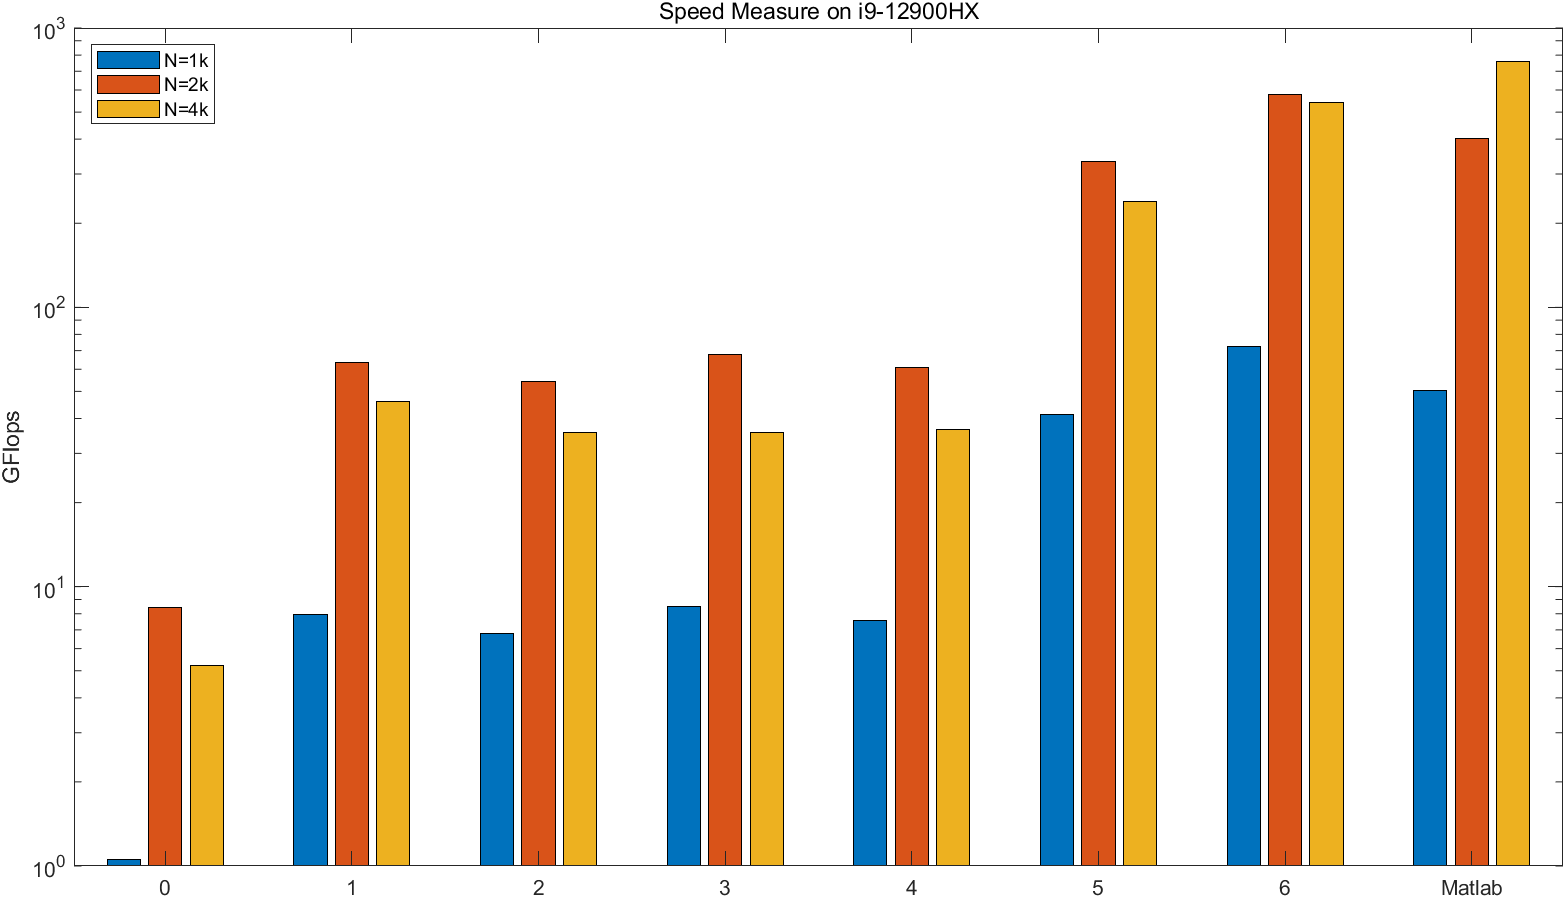
\includegraphics[width=0.8\textwidth]{improvement.png}
  \caption{Performance Camparion.} \label{fig:improvement}
\end{figure}
From the figure, we can see that the performance of the naive matrix multiplication algorithm is the worst. And the performance of different versions increases as the optimization level increases. The performance of the vectorized version is better than the naive version, and the performance of the blocked version is the best of all.
\subsection{Performance Camparion with Matlab}
For the blocked version, the performance is compared with the matrix multiplication algorithm in Matlab. The performance is compared in figure \ref{fig:matlab}
\begin{figure}[htbp]
  \centering
  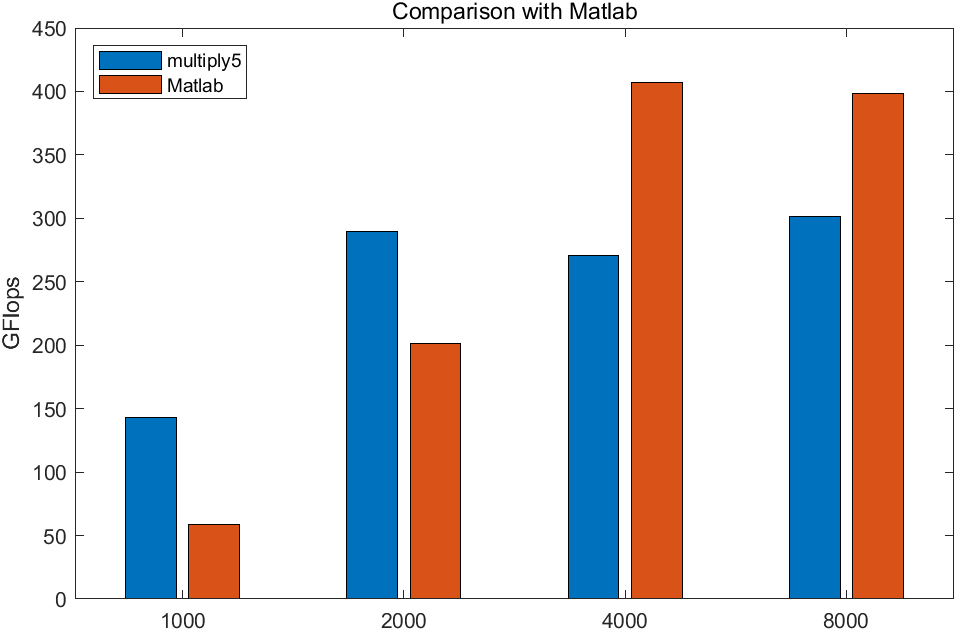
\includegraphics[width=0.8\textwidth]{vsmatlab.png}
  \caption{Performance Camparion with Matlab.} \label{fig:matlab}
\end{figure}
From the graph, we can see that the performance of the blocked version is close to the performance of the matrix multiplication algorithm in Matlab, and was able to beat Matlab when the matrix size is relatively small.
\section{Analysis}
Using Intel Advisor, we can analyze the performance of the our matrix multiplication algorithm. The performance of the block version is in figure \ref{fig:analysis}, here cluster QiMing was used, with 64 cores of \texttt{Intel(R) Xeon(R) Gold 6338 CPU @ 2.00GHz being used}

\begin{figure}[htbp]
  \centering
  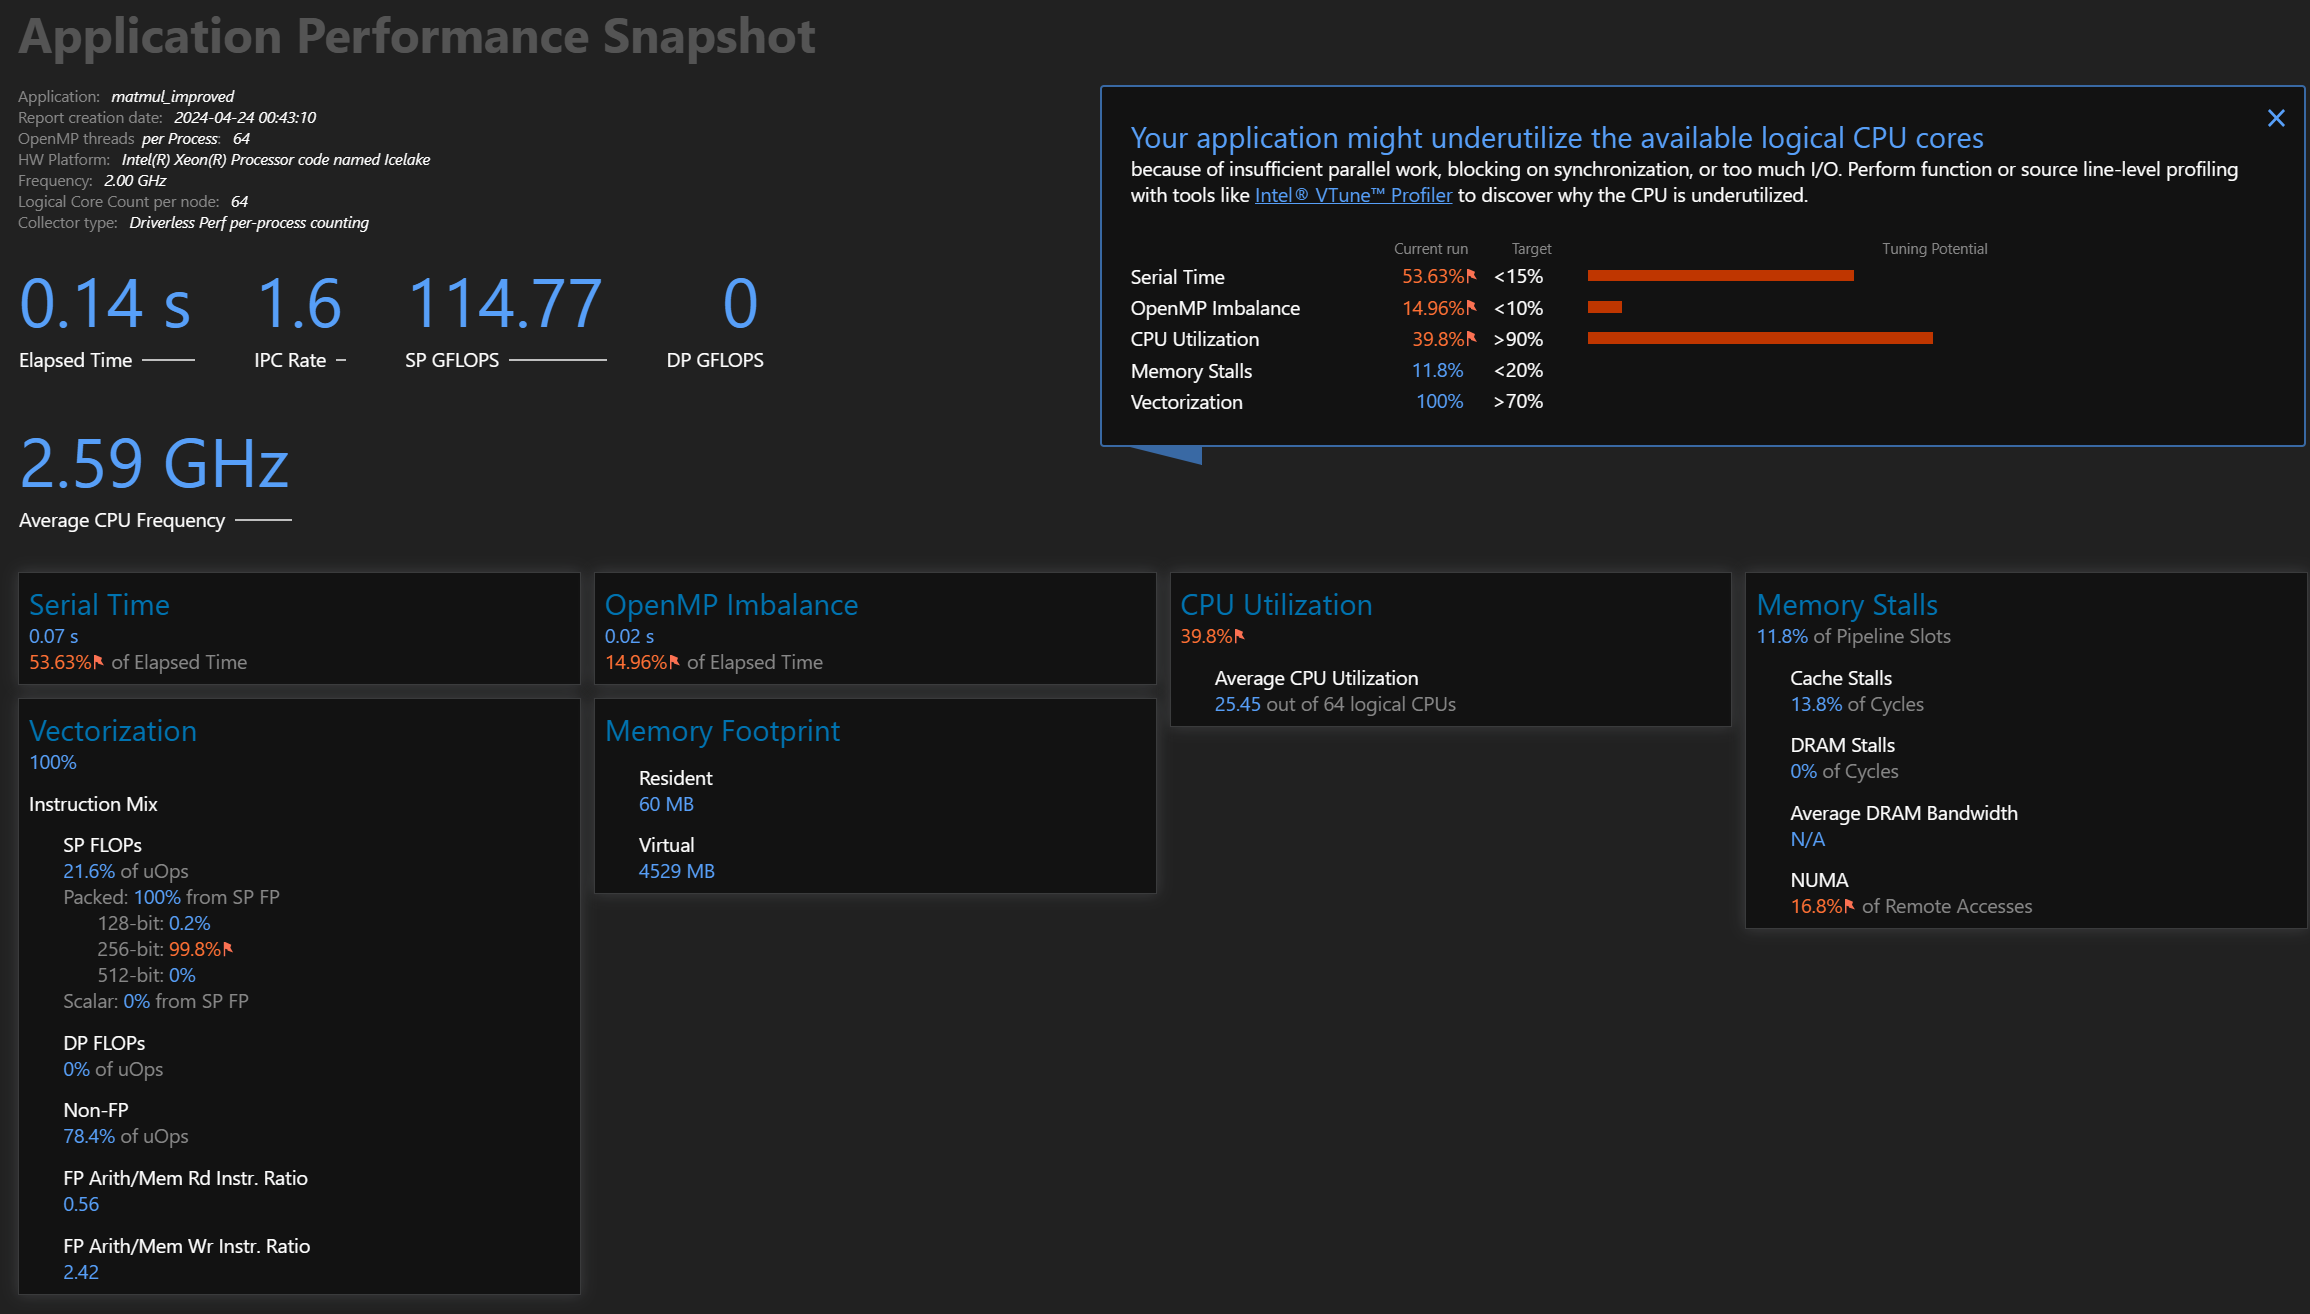
\includegraphics[width=0.8\textwidth]{profile1.png}
  \caption{Initial Profile for version 3.} \label{fig:analysis}
\end{figure}

As we can see, the profiler suggests that our CPU idles half of the time due to memory stall, and only half of the vector is used in the calculation. This is because 6638 supports AVX-512, which can calculate 16 floats at a time, while we only calculate 8 floats at a time. Thus we need to modify the code to calculate 16 floats at a time. The code is as follows:
\begin{lstlisting}[language=C,breaklines=true,basicstyle=\small,caption={AVX-512},captionpos=b]
  int multiply6(Matrix* A, Matrix* B, Matrix* C) {
    if (A->m != B->n) {
        printf("Error: Matrix dimensions do not match\n");
        return 1;
    }
    # pragma omp parallel for
    for (size_t jj = 0; jj <  C->n_pad; jj+=BLOCK\_SIZE) {
    for (size_t ii = 0; ii < C->m_pad; ii+=BLOCK\_SIZE*4) {
    for (size_t kk = 0; kk < A->m_pad; kk+=BLOCK\_SIZE) {
        for (size_t i = ii; i < ii + BLOCK\_SIZE*4; i+=16) {/*Loop over the columns of C */
        for (size_t j = jj; j < jj + BLOCK\_SIZE; j+=16) {/*Loow over the rows of C */
            // size_t b0_ptr = i;// b_ptr = i + k*B->m_pad
            // size_t b1_ptr = i + 1*B->m_pad;
            // size_t b2_ptr = i + 2*B->m_pad;
            // size_t b3_ptr = i + 3*B->m_pad;
            // size_t b4_ptr = i + 4*B->m_pad;
            // size_t b5_ptr = i + 5*B->m_pad;
            // size_t b6_ptr = i + 6*B->m_pad;
            // size_t b7_ptr = i + 7*B->m_pad;
            // size_t b8_ptr = i + 8*B->m_pad;
            // size_t b9_ptr = i + 9*B->m_pad;
            // size_t b10_ptr = i + 10*B->m_pad;
            // size_t b11_ptr = i + 11*B->m_pad;
            // size_t b12_ptr = i + 12*B->m_pad;
            // size_t b13_ptr = i + 13*B->m_pad;
            // size_t b14_ptr = i + 14*B->m_pad;
            // size_t b15_ptr = i + 15*B->m_pad;

            size_t bmpad = B->m_pad;
            __m512 b0, b1, b2, b3, b4, b5, b6, b7, b8, b9, b10, b11, b12, b13, b14, b15;
            __m512 a0, a1, a2, a3, a4, a5, a6, a7, a8, a9, a10, a11, a12, a13, a14, a15;
            __m512 c0 = _mm512_load_ps(&C->array[i/*:i+15*/ + j*C->m_pad]);
            __m512 c1 = _mm512_load_ps(&C->array[i + (j+1)*C->m_pad]);
            __m512 c2 = _mm512_load_ps(&C->array[i + (j+2)*C->m_pad]);
            __m512 c3 = _mm512_load_ps(&C->array[i + (j+3)*C->m_pad]);
            __m512 c4 = _mm512_load_ps(&C->array[i + (j+4)*C->m_pad]);
            __m512 c5 = _mm512_load_ps(&C->array[i + (j+5)*C->m_pad]);
            __m512 c6 = _mm512_load_ps(&C->array[i + (j+6)*C->m_pad]);
            __m512 c7 = _mm512_load_ps(&C->array[i + (j+7)*C->m_pad]);
            __m512 c8 = _mm512_load_ps(&C->array[i + (j+8)*C->m_pad]);
            __m512 c9 = _mm512_load_ps(&C->array[i + (j+9)*C->m_pad]);
            __m512 c10 = _mm512_load_ps(&C->array[i + (j+10)*C->m_pad]);
            __m512 c11 = _mm512_load_ps(&C->array[i + (j+11)*C->m_pad]);
            __m512 c12 = _mm512_load_ps(&C->array[i + (j+12)*C->m_pad]);
            __m512 c13 = _mm512_load_ps(&C->array[i + (j+13)*C->m_pad]);
            __m512 c14 = _mm512_load_ps(&C->array[i + (j+14)*C->m_pad]);
            __m512 c15 = _mm512_load_ps(&C->array[i + (j+15)*C->m_pad]);
            for (size_t k = kk; k < kk + BLOCK\_SIZE; k+=16) {
                size_t a_ptr;
                b0 = _mm512_load_ps(&B->array[i + k*B->m_pad]);// b_ptr = i + k*B->m_pad
                b1 = _mm512_load_ps(&B->array[i + (k+1)*B->m_pad]);
                b2 = _mm512_load_ps(&B->array[i + (k+2)*B->m_pad]);
                b3 = _mm512_load_ps(&B->array[i + (k+3)*B->m_pad]);
                b4 = _mm512_load_ps(&B->array[i + (k+4)*B->m_pad]);
                b5 = _mm512_load_ps(&B->array[i + (k+5)*B->m_pad]);
                b6 = _mm512_load_ps(&B->array[i + (k+6)*B->m_pad]);
                b7 = _mm512_load_ps(&B->array[i + (k+7)*B->m_pad]);
                b8 = _mm512_load_ps(&B->array[i + (k+8)*B->m_pad]);
                b9 = _mm512_load_ps(&B->array[i + (k+9)*B->m_pad]);
                b10 = _mm512_load_ps(&B->array[i + (k+10)*B->m_pad]);
                b11 = _mm512_load_ps(&B->array[i + (k+11)*B->m_pad]);
                b12 = _mm512_load_ps(&B->array[i + (k+12)*B->m_pad]);
                b13 = _mm512_load_ps(&B->array[i + (k+13)*B->m_pad]);
                b14 = _mm512_load_ps(&B->array[i + (k+14)*B->m_pad]);
                b15 = _mm512_load_ps(&B->array[i + (k+15)*B->m_pad]);

                # pragma unroll
                for (size_t l = 0; l < 16; l++) {
                    a_ptr = k + (j + l)*A->m_pad;
                    a0 = _mm512_set1_ps(A->array[a_ptr]);
                    a1 = _mm512_set1_ps(A->array[a_ptr + 1]);
                    a2 = _mm512_set1_ps(A->array[a_ptr + 2]);
                    a3 = _mm512_set1_ps(A->array[a_ptr + 3]);
                    a4 = _mm512_set1_ps(A->array[a_ptr + 4]);
                    a5 = _mm512_set1_ps(A->array[a_ptr + 5]);
                    a6 = _mm512_set1_ps(A->array[a_ptr + 6]);
                    a7 = _mm512_set1_ps(A->array[a_ptr + 7]);
                    a8 = _mm512_set1_ps(A->array[a_ptr + 8]);
                    a9 = _mm512_set1_ps(A->array[a_ptr + 9]);
                    a10 = _mm512_set1_ps(A->array[a_ptr + 10]);
                    a11 = _mm512_set1_ps(A->array[a_ptr + 11]);
                    a12 = _mm512_set1_ps(A->array[a_ptr + 12]);
                    a13 = _mm512_set1_ps(A->array[a_ptr + 13]);
                    a14 = _mm512_set1_ps(A->array[a_ptr + 14]);
                    a15 = _mm512_set1_ps(A->array[a_ptr + 15]);
                    c0 = _mm512_fmadd_ps(a0, b0, c0);
                    c1 = _mm512_fmadd_ps(a1, b1, c1);
                    c2 = _mm512_fmadd_ps(a2, b2, c2);
                    c3 = _mm512_fmadd_ps(a3, b3, c3);
                    c4 = _mm512_fmadd_ps(a4, b4, c4);
                    c5 = _mm512_fmadd_ps(a5, b5, c5);
                    c6 = _mm512_fmadd_ps(a6, b6, c6);
                    c7 = _mm512_fmadd_ps(a7, b7, c7);
                    c8 = _mm512_fmadd_ps(a8, b8, c8);
                    c9 = _mm512_fmadd_ps(a9, b9, c9);
                    c10 = _mm512_fmadd_ps(a10, b10, c10);
                    c11 = _mm512_fmadd_ps(a11, b11, c11);
                    c12 = _mm512_fmadd_ps(a12, b12, c12);
                    c13 = _mm512_fmadd_ps(a13, b13, c13);
                    c14 = _mm512_fmadd_ps(a14, b14, c14);
                    c15 = _mm512_fmadd_ps(a15, b15, c15);
                    
                }
            }
            _mm512_store_ps(&C->array[i/*:i+15*/ + j*C->m_pad], c0);
            _mm512_store_ps(&C->array[i + (j+1)*C->m_pad], c1);
            _mm512_store_ps(&C->array[i + (j+2)*C->m_pad], c2);
            _mm512_store_ps(&C->array[i + (j+3)*C->m_pad], c3);
            _mm512_store_ps(&C->array[i + (j+4)*C->m_pad], c4);
            _mm512_store_ps(&C->array[i + (j+5)*C->m_pad], c5);
            _mm512_store_ps(&C->array[i + (j+6)*C->m_pad], c6);
            _mm512_store_ps(&C->array[i + (j+7)*C->m_pad], c7);
            _mm512_store_ps(&C->array[i + (j+8)*C->m_pad], c8);
            _mm512_store_ps(&C->array[i + (j+9)*C->m_pad], c9);
            _mm512_store_ps(&C->array[i + (j+10)*C->m_pad], c10);
            _mm512_store_ps(&C->array[i + (j+11)*C->m_pad], c11);
            _mm512_store_ps(&C->array[i + (j+12)*C->m_pad], c12);
            _mm512_store_ps(&C->array[i + (j+13)*C->m_pad], c13);
            _mm512_store_ps(&C->array[i + (j+14)*C->m_pad], c14);
            _mm512_store_ps(&C->array[i + (j+15)*C->m_pad], c15);
        }
        }
    }                          
    }
    }
    return 0;
}
\end{lstlisting}
In the code, \texttt{\# pragma unroll} is used to unroll the loop, and \texttt{\_mm512\_set1\_ps} is used to set a vector with the same value, and \texttt{\_mm512\_load\_ps} is used to load a vector from memory. The \texttt{\_mm512\_fmadd\_ps} function is used to multiply and add two vectors. The code is then compiled with the \texttt{-mavx512f} flag.

What is more, althogh the \texttt{BLOCK\_SIZE} is set to set to 32 in the begining, experiments show that the performance is better when \texttt{BLOCK\_SIZE} is set to 64, for $N=16\times10^3$, the calculation time is 6.783168s for \texttt{BLOCK\_SIZE}=32, and 3.454644s for \texttt{BLOCK\_SIZE=64}, that is, the tuning of \texttt{BLOCK\_SIZE} is also important. Also, the performance of the algorithm seems to be better when the outermost loop is over the rows of C, this is because the matrix is stored in column major, and the cache is more friendly when the outermost loop is over the rows of $C$. 

After tuning the code, we can test the performance of the code on $N=6.4\times10^4$, the performance of the code is in figure \ref{fig:analysis2}
Now the performance of the code is in figure \ref{fig:analysis2}
\begin{figure}[htbp]
  \centering
  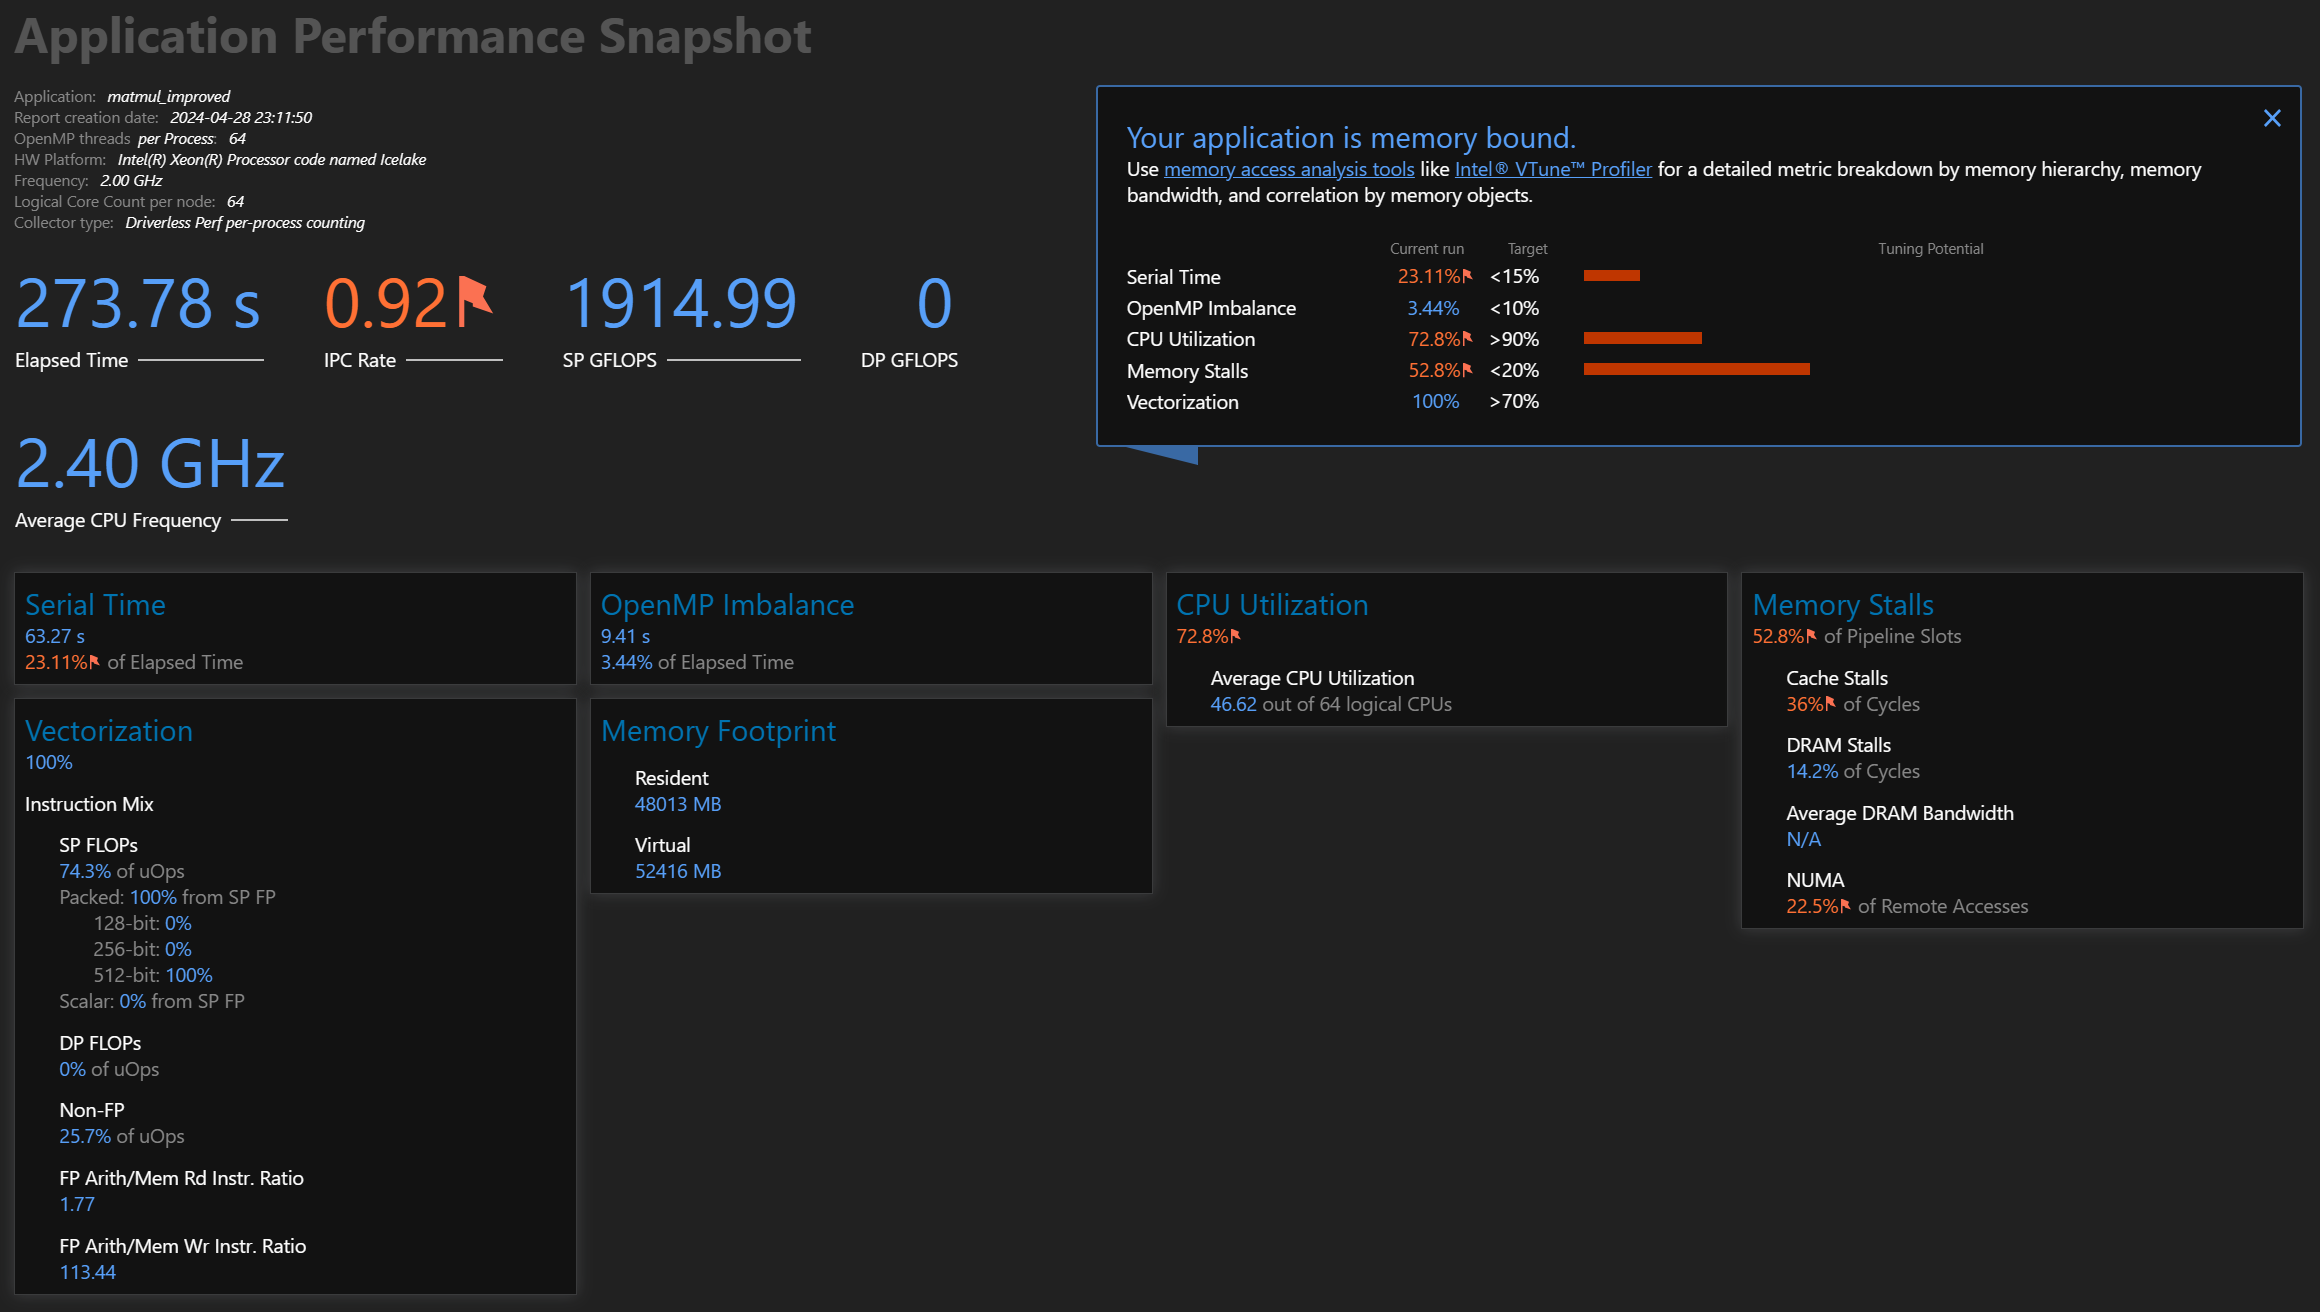
\includegraphics[width=0.8\textwidth]{profile2.png}
  \caption{Profile for version 6} \label{fig:analysis2}
\end{figure}
Since the aps also include the time for memory allocation, and the output time for calculation is 228.714687s, the actual performance of the code is 2.29TFlops, with the CPU idling less then 25\% of the time.

\section{Conclusion}
In this project, we implemented a matrix multiplication algorithm in C, and optimized the algorithm using vectorization, loop unrolling, and blocking. The performance of the different algorithms was compared, and the blocked version was able to beat Matlab when the matrix size is relatively small. The performance of the blocked version was further improved by using AVX-512, and the performance of the code was close to the performance of the matrix multiplication algorithm in Matlab. 

\section{Appendix}
\subsection{Original Data and Code for Ploting}
\begin{verbatim}
  Time1k = [0.229796;
  0.043154;
  0.037065;
  0.031924;
  0.034419;
  0.007962;
  0.007007;0.017011];
  
  Time2k = [1.902727;
  0.252489;
  0.293857;
  0.235492;
  0.263778;
  0.048274;
  0.027653;0.039786];
  Time4k = [24.561001;
  2.781965;
  3.583504;
  3.580928;
  3.505939;
  0.535964;
  0.236099;0.168062];
  bar([2*1e3^3./Time2k,2*2e3^3./Time2k,2*4e3^3./Time4k]./1e9)
  set(gca, 'XTickLabel',{0,1,2,3,4,5,6,'Matlab'})
  set(gca,'YScale','log')
  legend('N=1k','N=2k','N=4k',Location='northwest')
  ylabel('GFlops')
  title('Speed Measure on i9-12900HX')
  timeVSMatlab = [0.007007,0.017011;
 0.027653,0.039786;
 0.236099,0.168062;
  1.662961,1.471775];
matSize = repmat([1;2;4;8]*1e3,1,2);
bar(matSize.^3./timeVSMatlab/1e9)
set(gca, 'XTickLabel',[1;2;4;8]*1e3)
legend('multiply5','Matlab',Location='northwest')
ylabel('GFlops')
title('Comparison with Matlab')
\end{verbatim}
\end{document}